\begin{figure}[t]
  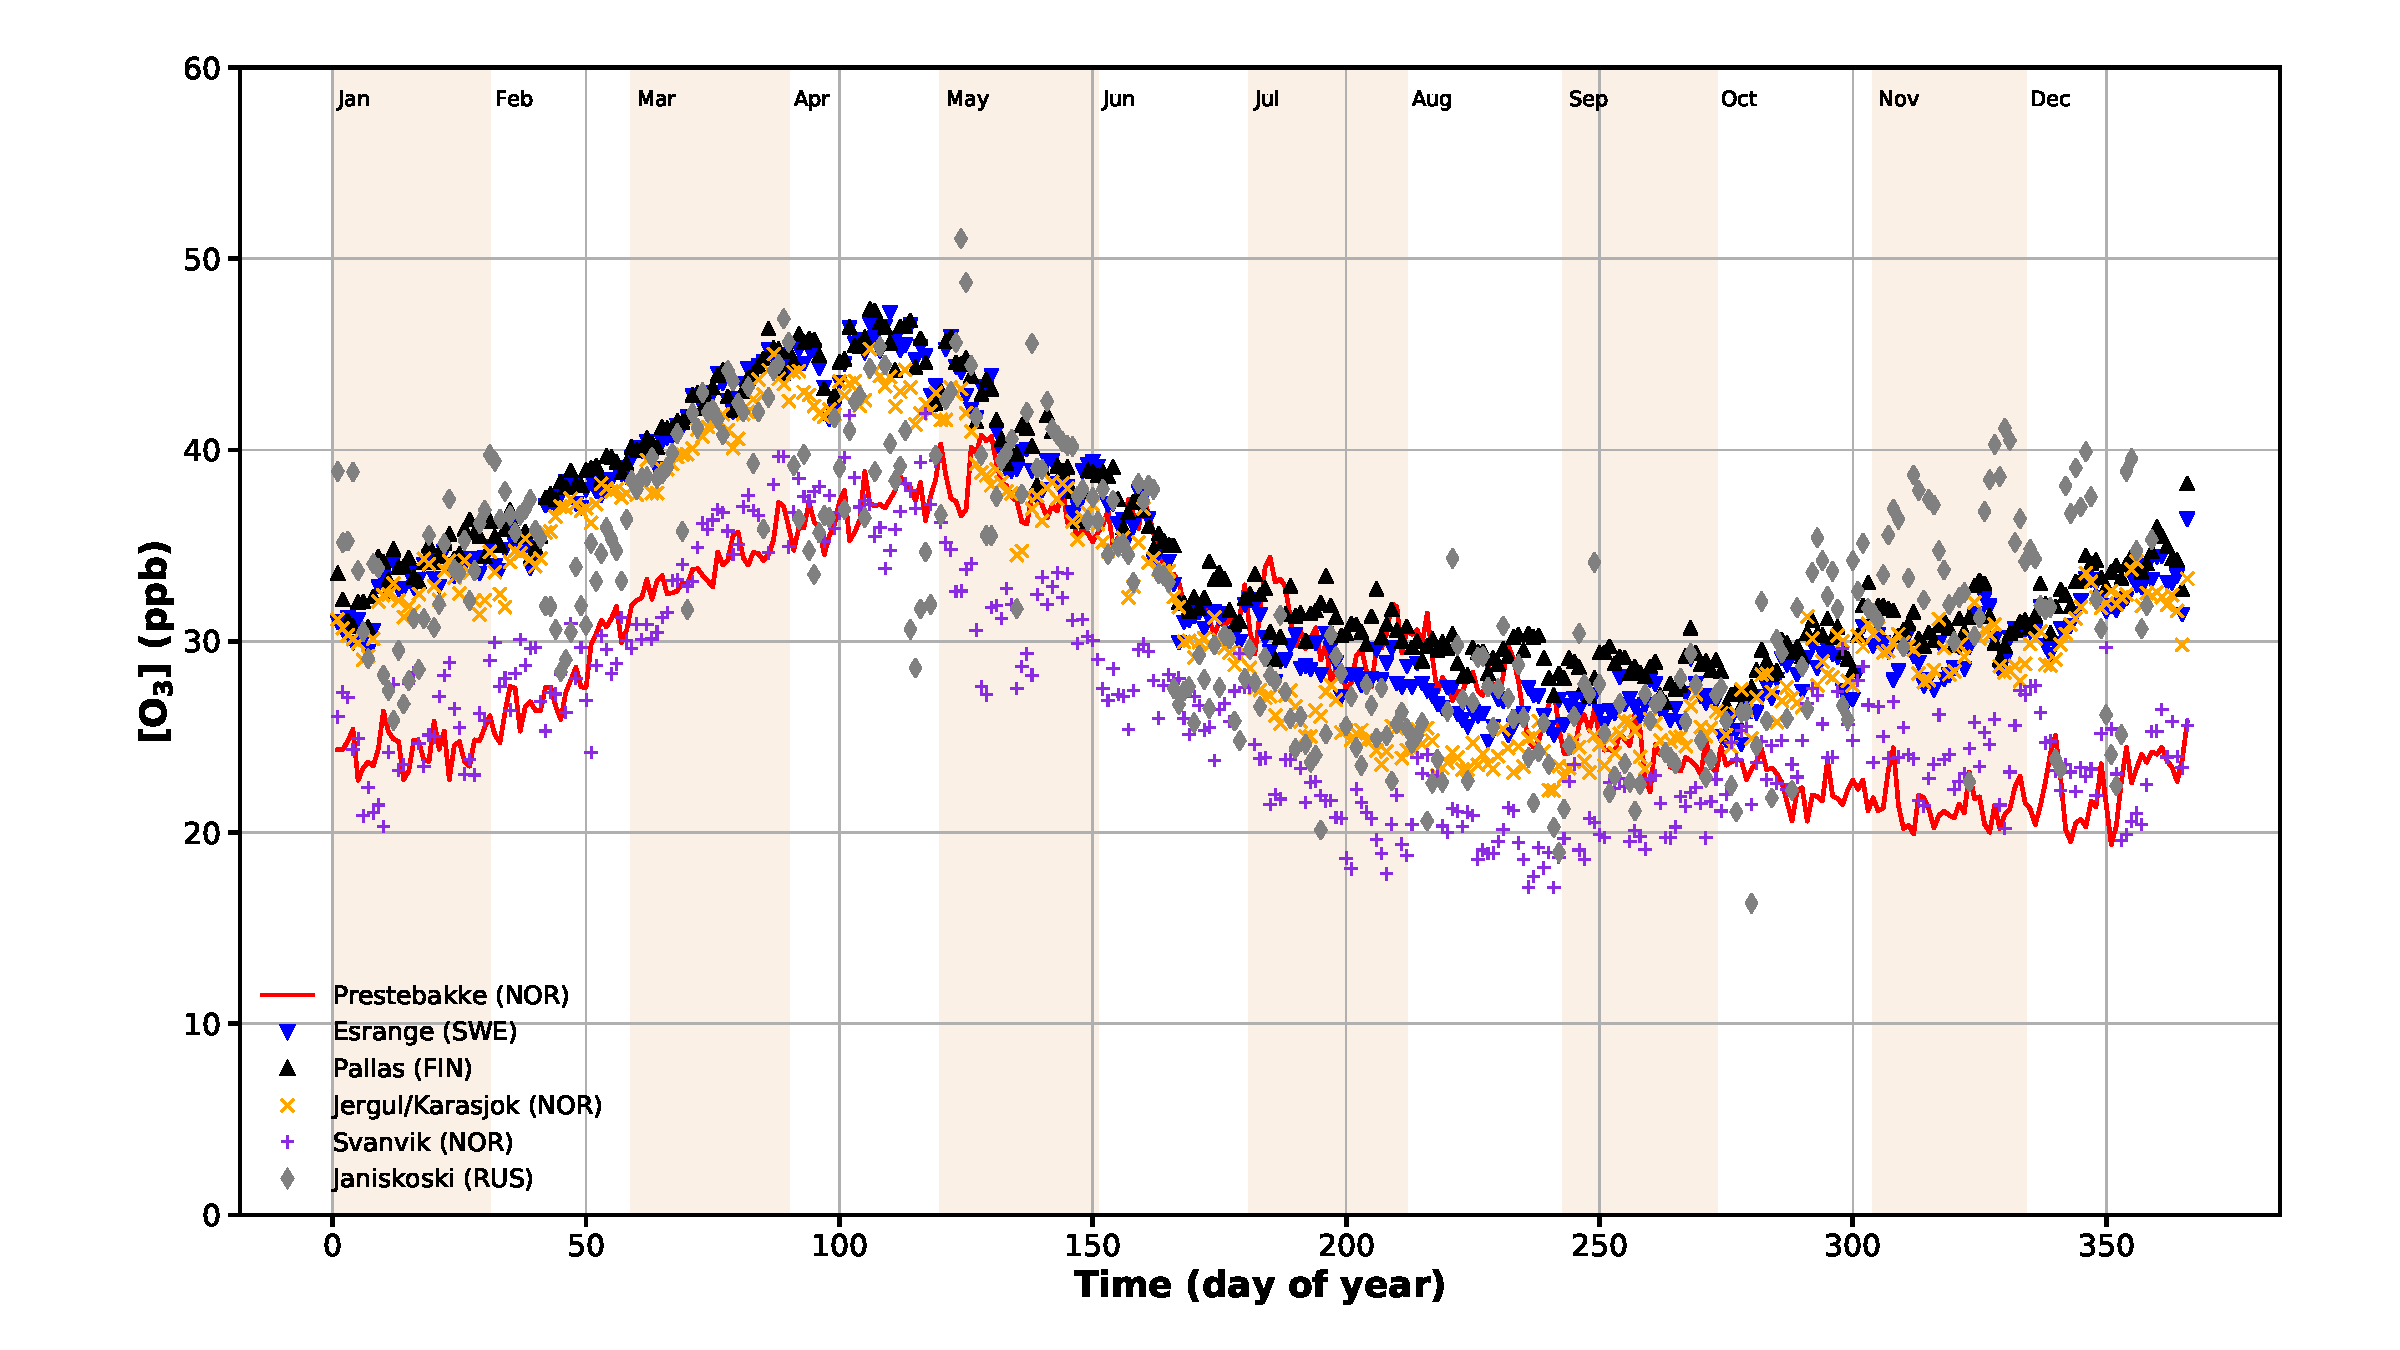
\includegraphics[width=8.3cm]{ozone_climatology_fenoscandic_obs}
  \caption{S1 Multi-annual mean of daily mean ozone at observation sites in Fennoscandia. The large spread in case of Svanvik and Janiskoski is due to the lower statistics. All climatologies peak in spring, with peak values in April. The annual average ozone concentration \chem{\left<[O_3]\right>} at Svanvik is $6.6\,\unit{ppb}$ lower than at the sites at Jergul/Karasjok (NOR), Esrange (SWE), and Pallas (FIN).}
  \label{fig:ozone_climatology_fenoscandic_obs}
\end{figure}
